\section{问题三：轮廓压缩与线长优化模型的建立与求解}

问题三将问题二的固定死区率推广为正方形整数边长搜索。本文先利用面积与模块尺寸确定轮廓下界，再按边长逐一构造布局，并在当前搜索策略首次成功构造全部模块的边长下复用问题二的网络驱动优化，由此考察死区率下降所带来的 HPWL 代价。

\subsection{轮廓压缩的词典序模型}

\subsubsection{面积下界、模块下界与搜索边长}

设全部硬模块的总面积为
\begin{equation}
  A_{\mathrm{block}}=\sum_i w_i^0h_i^0.
  \label{eq:q3_block_area}
\end{equation}
若正方形轮廓边长为整数 $S$，则面积必要条件和单模块尺寸必要条件分别给出
\begin{equation}
  S_{\mathrm{area}}=\left\lceil\sqrt{A_{\mathrm{block}}}\right\rceil,
  \qquad
  S_{\mathrm{block}}=\max_i\max(w_i^0,h_i^0),
  \label{eq:q3_lower_bounds}
\end{equation}
从而搜索下界为
\begin{equation}
  S_{\mathrm{lb}}=\max\left(S_{\mathrm{area}},S_{\mathrm{block}}\right).
  \label{eq:q3_search_lb}
\end{equation}
三组实例的下界分解以及问题二提供的已知可行边长上界见表~\ref{tab:q3_search_bounds}。

\begin{table}[H]
  \centering
  \caption{问题三整数轮廓边长的搜索区间}
  \label{tab:q3_search_bounds}
  \small
  \renewcommand{\arraystretch}{1.15}
  \begin{tabular}{c r r r r r}
    \toprule
    实例 & $A_{\mathrm{block}}$ & $S_{\mathrm{area}}$ & $S_{\mathrm{block}}$ & $S_{\mathrm{lb}}$ & 问题二整数上界 \\
    \midrule
    \texttt{n100} & 179501 & 424 & 67 & 424 & 454 \\
    \texttt{n200} & 175696 & 420 & 48 & 420 & 449 \\
    \texttt{n300} & 273170 & 523 & 48 & 523 & 560 \\
    \bottomrule
  \end{tabular}
\end{table}

对于任一候选边长 $S\ge S_{\mathrm{lb}}$，旋转后的模块宽高仍由式~(\ref{eq:q1_rotation}) 确定，并满足
\begin{equation}
  0\le x_i,\quad 0\le y_i,\quad
  x_i+w_i\le S,\quad y_i+h_i\le S,
  \label{eq:q3_boundary}
\end{equation}
以及式~(\ref{eq:q1_nonoverlap}) 的两两非重叠约束。

\subsubsection{死区率与词典序目标}

候选边长 $S$ 对应的死区率为
\begin{equation}
  \Gamma(S)=\frac{S^2-A_{\mathrm{block}}}{A_{\mathrm{block}}}.
  \label{eq:q3_deadspace}
\end{equation}
由于 $A_{\mathrm{block}}$ 固定，$\Gamma(S)$ 随 $S$ 严格单调增加，故最小化死区率等价于最小化 $S$。题目优化顺序是先压缩轮廓、再控制线长，因此以式~(\ref{eq:q2_total_hpwl}) 定义的总 HPWL $\mathcal{L}$ 为第二层目标，建立
\begin{equation}
  \operatorname{lexmin}\left(S,\mathcal{L}\right),
  \quad
  \text{s.t. 式~(\ref{eq:q3_boundary}) 和式~(\ref{eq:q1_nonoverlap})成立}.
  \label{eq:q3_lex_model}
\end{equation}
这一目标保持了题目给定的优先级，也避免为面积与线长人为设置权重。

本文将轮廓解释为硬模块的摆放边界：固定 Terminal 仅作为网络引脚参与 HPWL，不计入硬模块面积，也不受该边界约束。该解释下，问题三的主模型依次由 $A_{\mathrm{block}}$、$S_{\mathrm{area}}$ 与 $S_{\mathrm{block}}$、$S_{\mathrm{lb}}$、候选 $S$、$\Gamma(S)$ 和 $\operatorname{lexmin}(S,\mathcal{L})$ 构成；替代题意口径在第 9 节进行敏感性分析，相应诊断计数列于附录 A.2。

\subsection{整数边长搜索与网络驱动优化}

\subsubsection{从理论下界逐整数搜索轮廓}

对每组实例，从 $S_{\mathrm{lb}}$ 到问题二的整数合法化边界逐一枚举 $S$。在每个边长下，组合 MaxRects 的最短边适配、面积适配和最长边适配规则，以及面积、长边、短边和长宽比四种模块排序方式，并允许模块旋转；仅当全部模块均被放入 $S\times S$ 轮廓时，才记录该边长并终止外层搜索。

MaxRects 不是装箱可行性的完备判定器：小于 $S_{\mathrm{found}}$ 的边长未成功构造布局，只说明当前启发式策略搜索失败，不能证明数学不可行。因此，$S_{\mathrm{found}}$ 统一称为“当前搜索策略获得的最小成功构造边长”。

\subsubsection{成功构造边长下复用问题二的线长优化}

固定 $S=S_{\mathrm{found}}$ 后，继续采用问题二的 HPWL 优化方法：先由二次线长松弛求得模块目标中心，再通过行带构造和目标引导合法化生成确定性初始布局，按初始 HPWL 选取前 $3$ 个候选进行两轮单模块局部重插入。其中，\texttt{n100} 使用精确空矩形重插入，\texttt{n200} 与 \texttt{n300} 使用 HPWL 断点搜索，最终按复算后的 HPWL 选择布局。该过程保持整数边长搜索、MaxRects 策略和问题二线长优化方法不变。

\subsection{死区率---HPWL 权衡结果与机制分析}

三组实例的轮廓压缩与线长结果见表~\ref{tab:q3_main_results}。当前搜索策略获得的最小成功构造边长分别为 $439$、$432$、$537$；相较问题二统一设定的 $15\%$ 死区率，问题三将死区率压缩至 $7.3649\%$、$6.2198\%$、$5.5639\%$。与此同时，总 HPWL 分别由 $220279.0$、$410072.5$、$560492.5$ 增至 $239551.0$、$442024.0$、$640695.5$，相对增加约 $8.75\%$、$7.79\%$、$14.31\%$。

\begin{table}[H]
  \centering
  \caption{问题三轮廓压缩与 HPWL 权衡结果}
  \label{tab:q3_main_results}
  \small
  \renewcommand{\arraystretch}{1.15}
  \begin{tabular}{c r r r r r r}
    \toprule
    实例 & $S_{\mathrm{lb}}$ & $S_{\mathrm{found}}$ & 死区率/\% & 问题二 HPWL & 问题三 HPWL & 增量/\% \\
    \midrule
    \texttt{n100} & 424 & 439 & 7.3649 & 220279.0 & 239551.0 & 8.7489 \\
    \texttt{n200} & 420 & 432 & 6.2198 & 410072.5 & 442024.0 & 7.7917 \\
    \texttt{n300} & 523 & 537 & 5.5639 & 560492.5 & 640695.5 & 14.3094 \\
    \bottomrule
  \end{tabular}
\end{table}

为使面积利用率改善与互连代价处于同一视觉主线上，图~\ref{fig:q3_tradeoff} 分别绘制问题二到问题三的死区率变化和以问题二为基准的 HPWL 指数变化。

\begin{figure}[H]
  \centering
  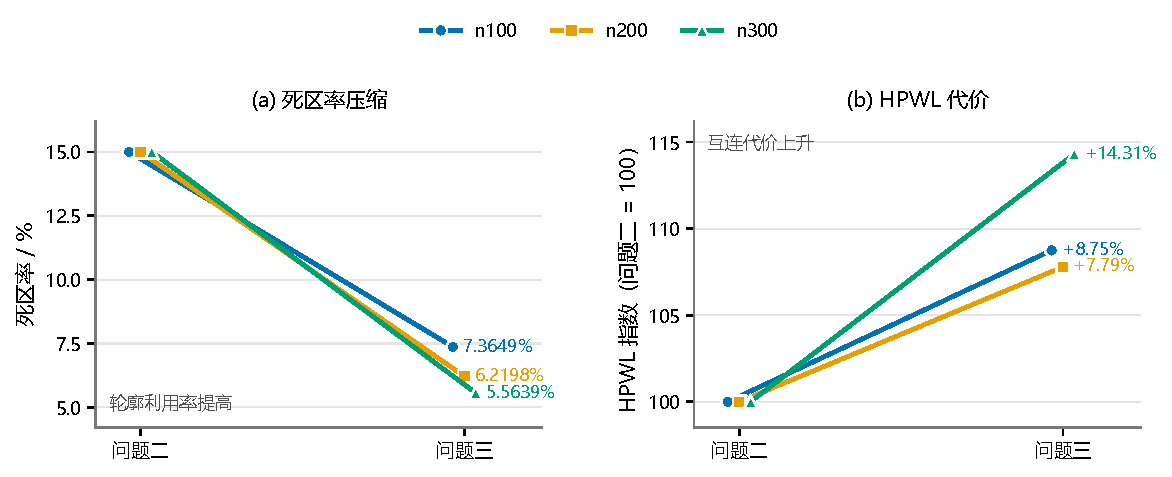
\includegraphics[width=0.88\textwidth]{../results/q3/figures/q3_tradeoff_q2_q3.pdf}
  \caption{问题二到问题三的死区率压缩与 HPWL 增长关系}
  \label{fig:q3_tradeoff}
\end{figure}

图~\ref{fig:q3_tradeoff} 左侧三条线均明显下降，而右侧三条线同时上升，直接呈现“更低死区率---更高互连线长”的权衡。轮廓压缩减少了可供模块平移、旋转和重插入的空隙，也限制了模块围绕网络目标中心调整的空间；因此，几何利用率提高的代价是互连结构受到更强的空间约束，网络外接框难以同时收缩，最终表现为总 HPWL 上升。这一变化是词典序目标先满足轮廓压缩所产生的结果，而非单一线长优化阶段的失效。

在三组实例中，\texttt{n300} 的 HPWL 增幅最大。结果表明其对空间压缩更敏感；结合该实例更大的模块与网络规模，这一现象提示：当更多模块和网络共同竞争有限的调整空间时，紧轮廓可能更快削弱线长优化的自由度，但该观察仅限于当前三组算例。

固定最小成功构造边长后，两轮局部搜索分别保留 $89$、$81$、$69$ 次有效移动，并将 HPWL 从 $244183.0$、$442742.5$、$644858.0$ 降至表~\ref{tab:q3_main_results} 所列结果，说明紧轮廓内仍有局部改善空间。对应布局见图~\ref{fig:q3_n100_n200} 和图~\ref{fig:q3_n300}。

\begin{figure}[H]
  \centering
  \begin{minipage}[t]{0.48\textwidth}
    \centering
    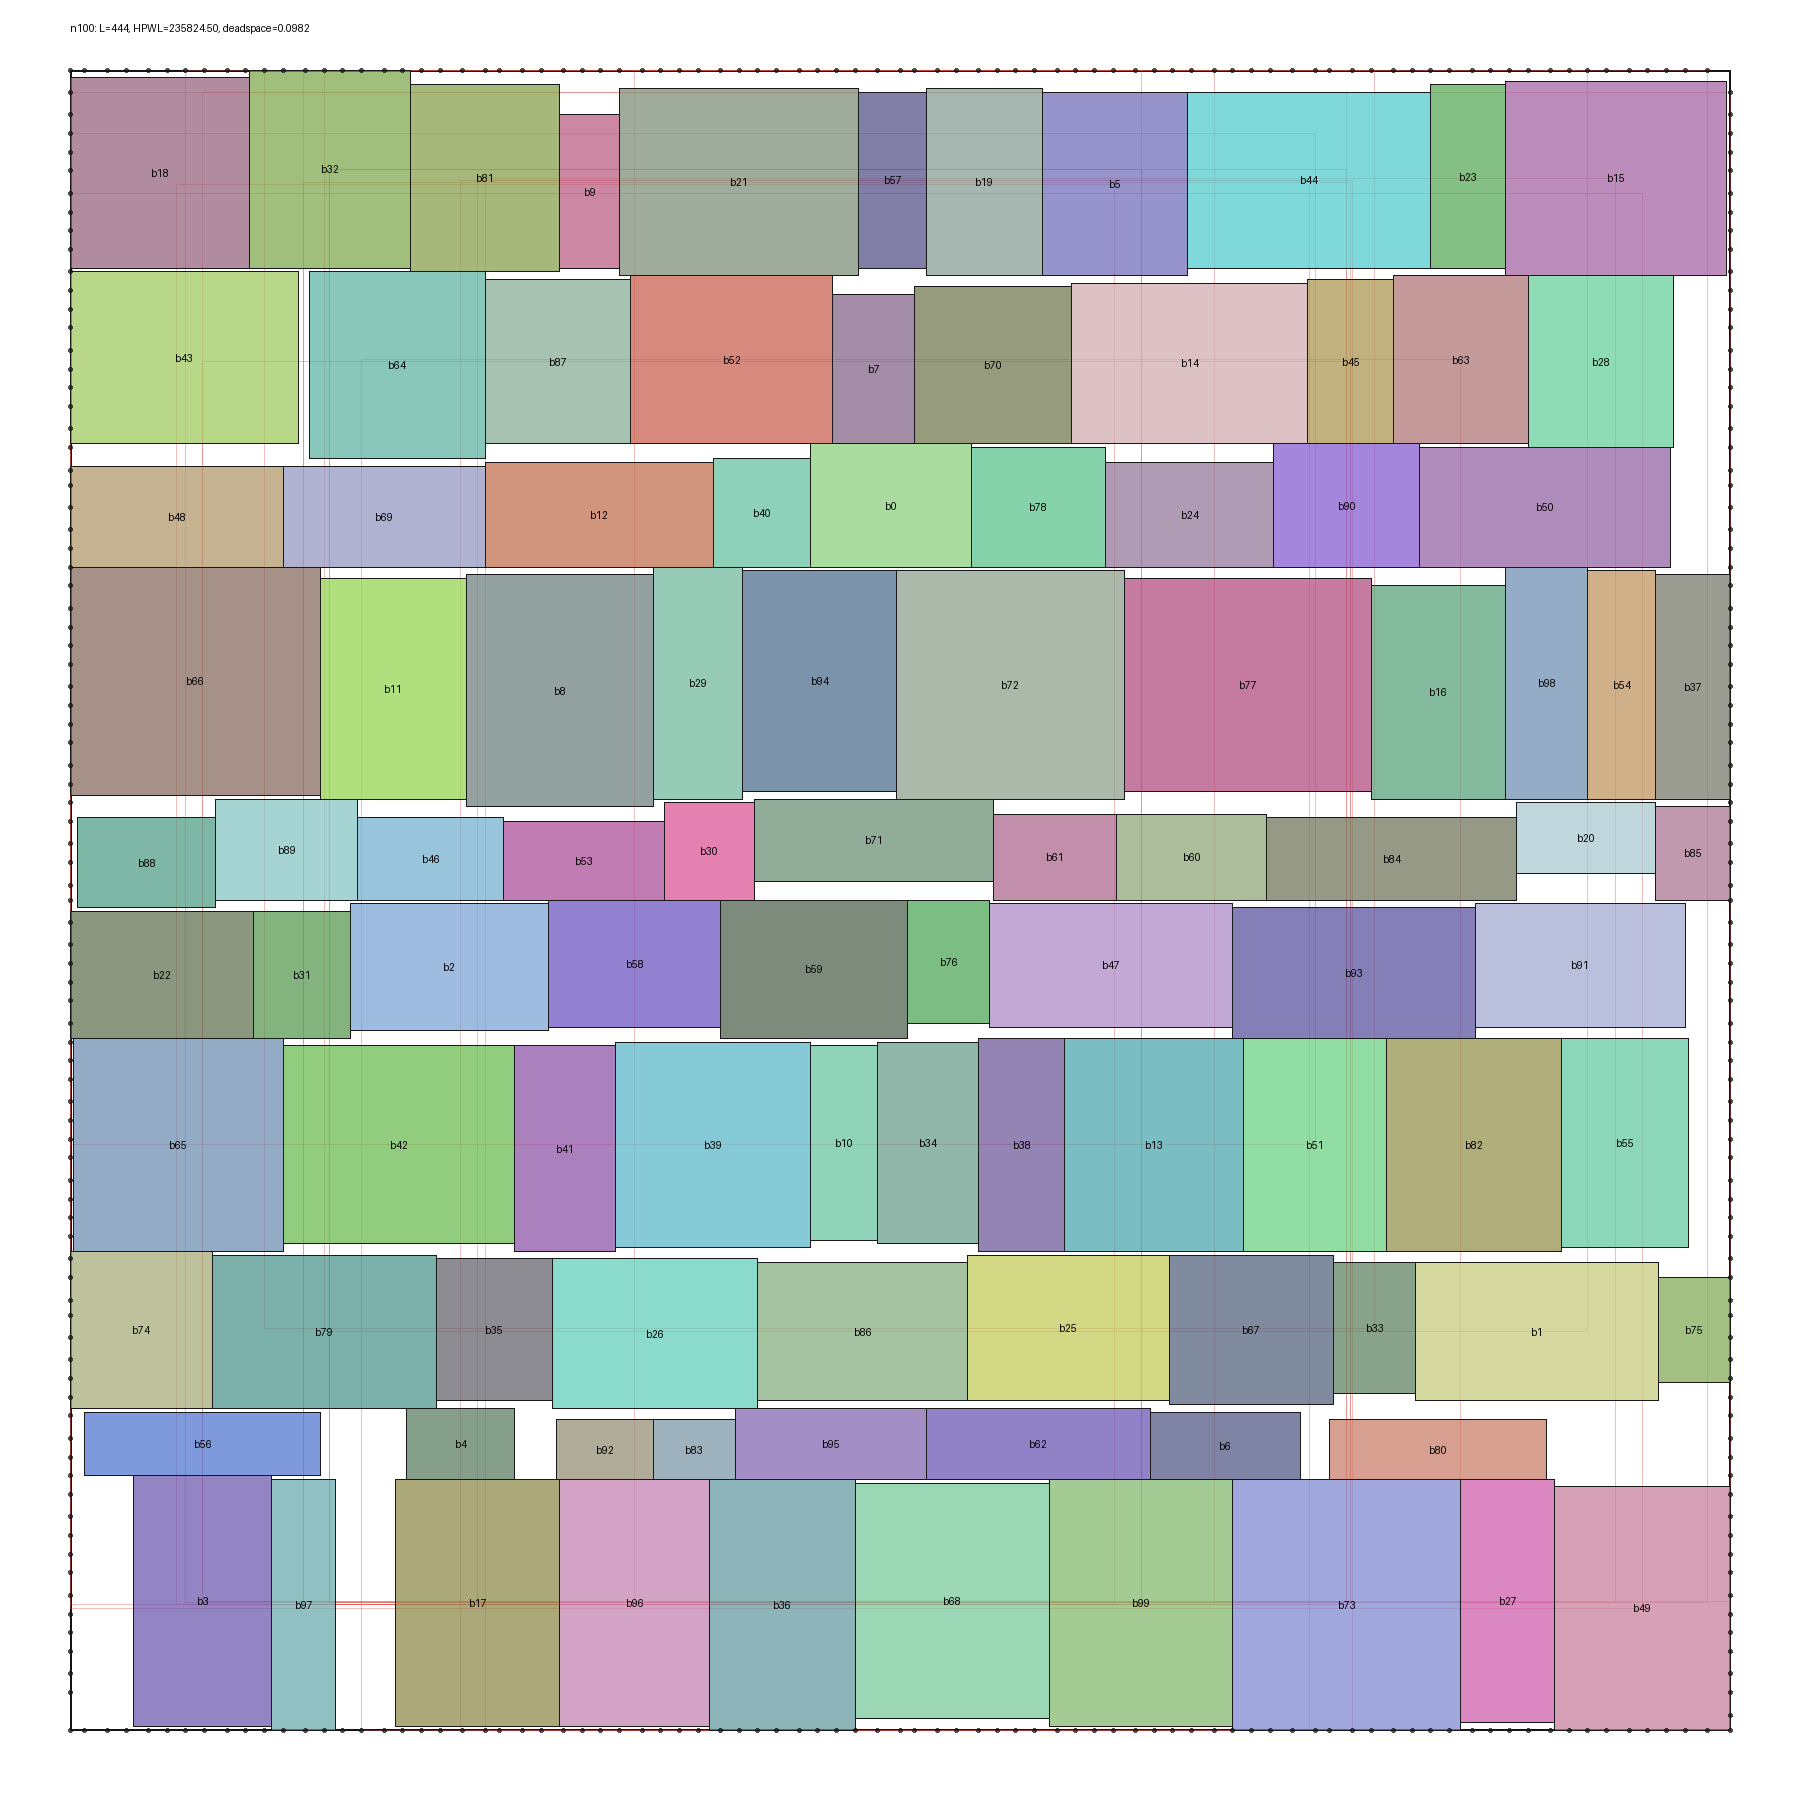
\includegraphics[width=\textwidth]{../results/q3/figures/n100_q3_layout.png}\\[-0.3em]
    {\small (a) \texttt{n100}}
  \end{minipage}
  \hfill
  \begin{minipage}[t]{0.48\textwidth}
    \centering
    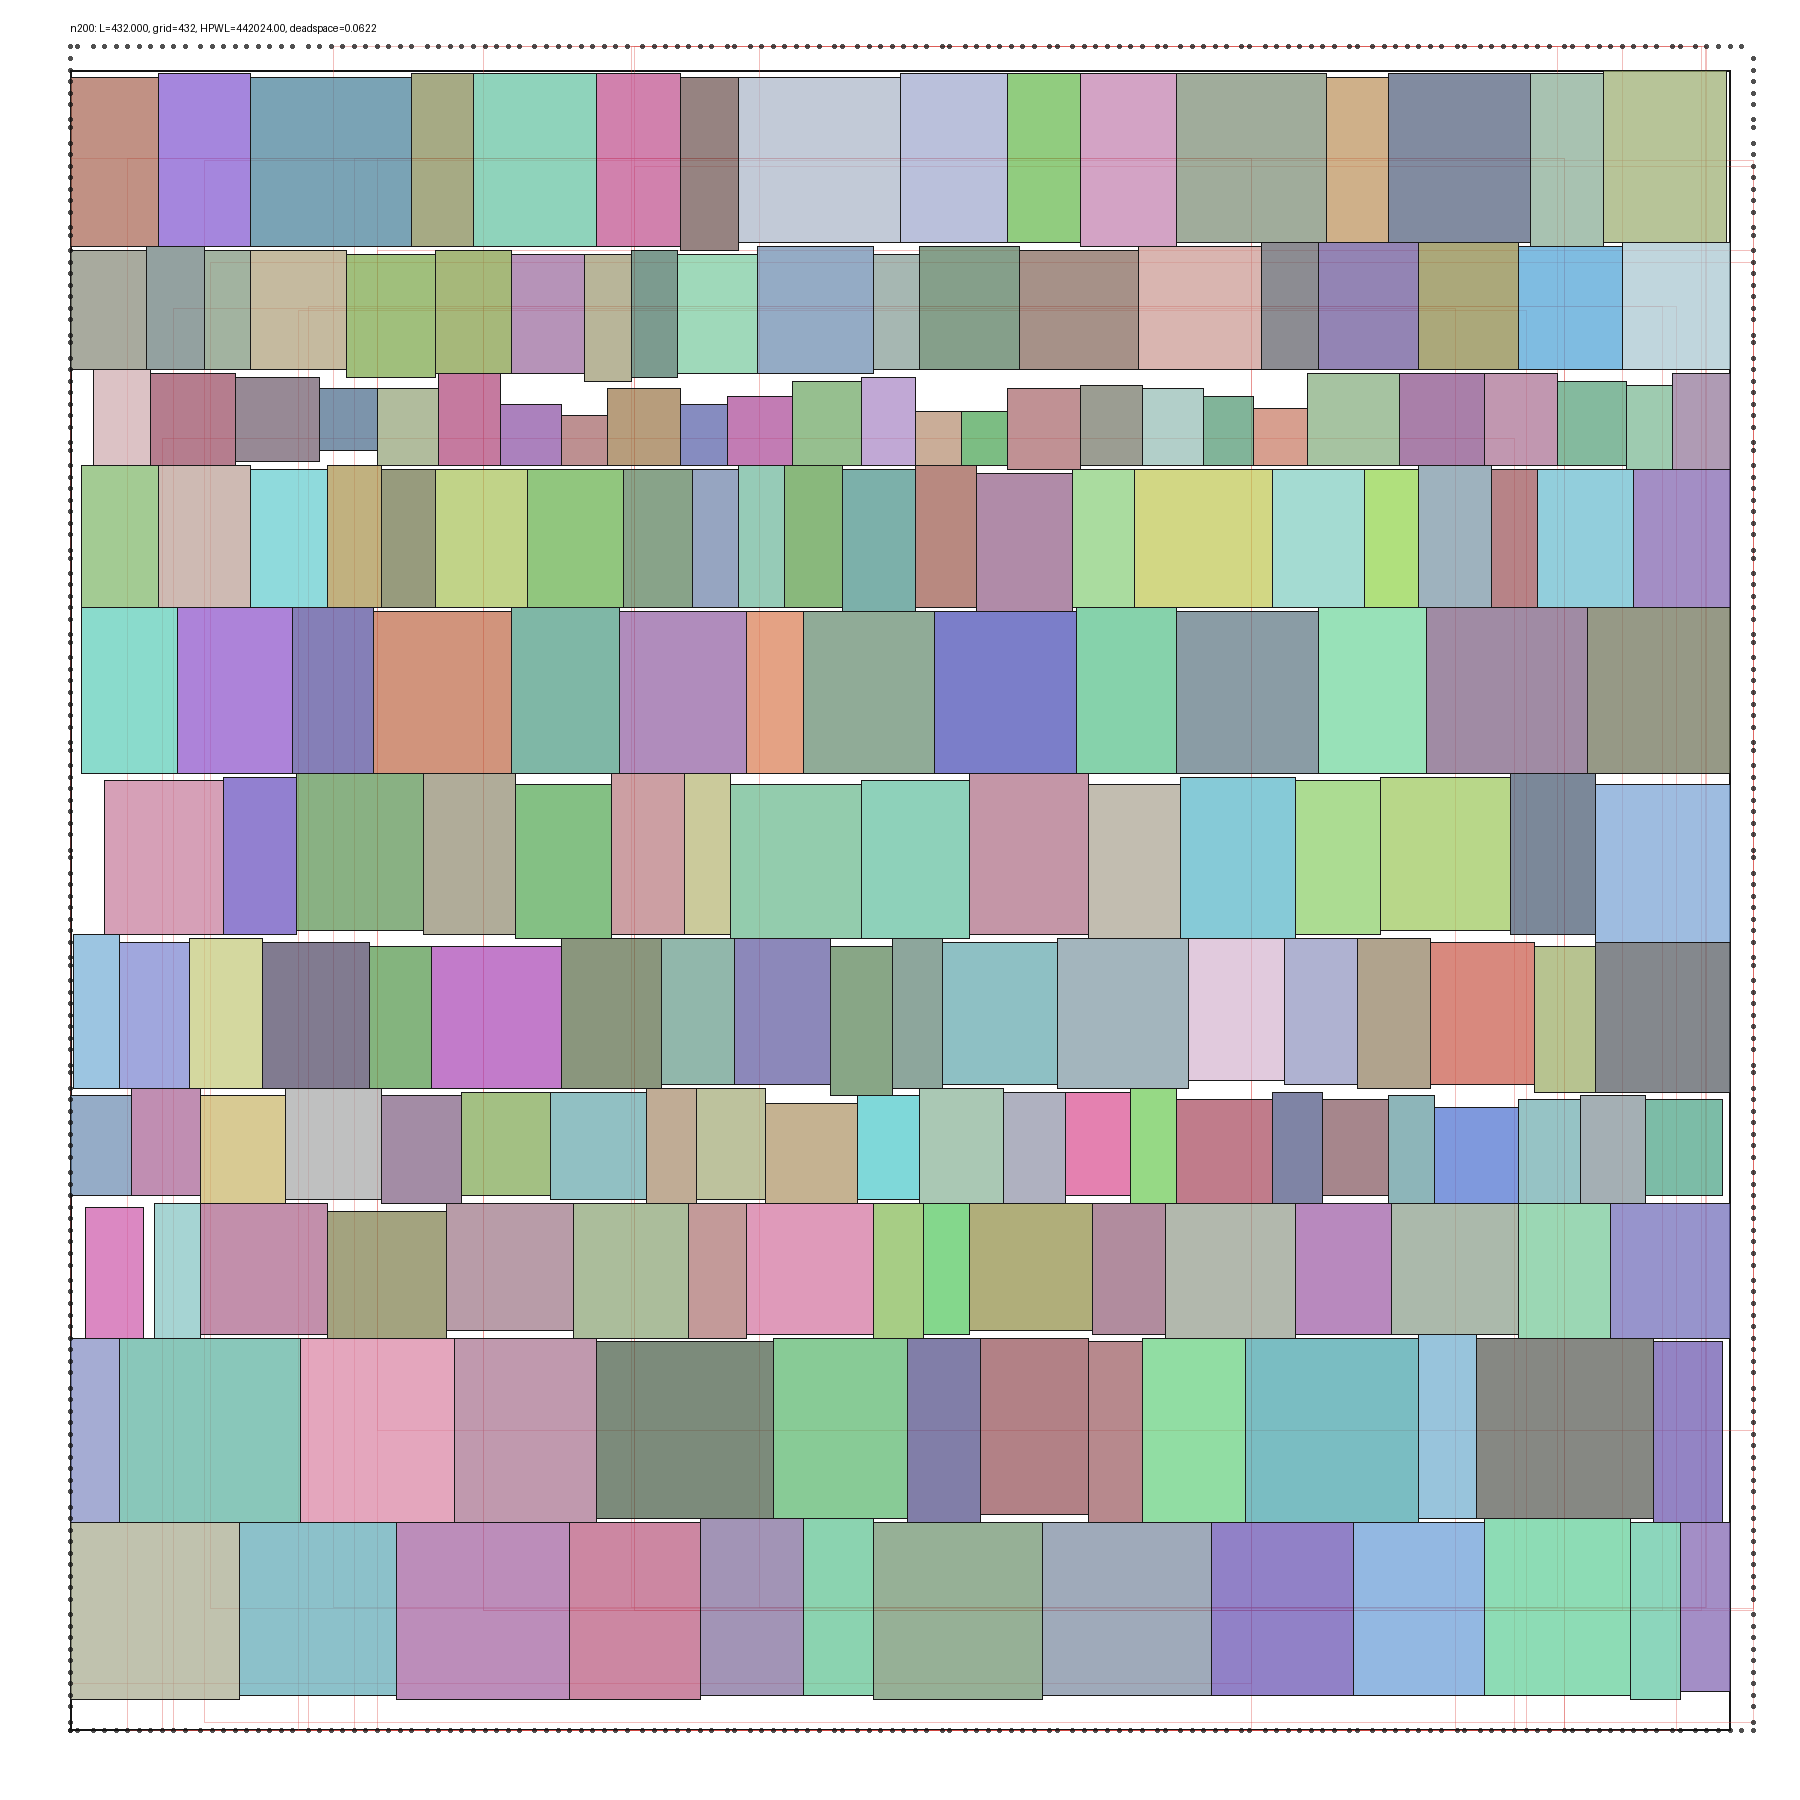
\includegraphics[width=\textwidth]{../results/q3/figures/n200_q3_layout.png}\\[-0.3em]
    {\small (b) \texttt{n200}}
  \end{minipage}
  \caption{问题三 \texttt{n100} 与 \texttt{n200} 的紧轮廓硬模块布局}
  \label{fig:q3_n100_n200}
\end{figure}

\begin{figure}[H]
  \centering
  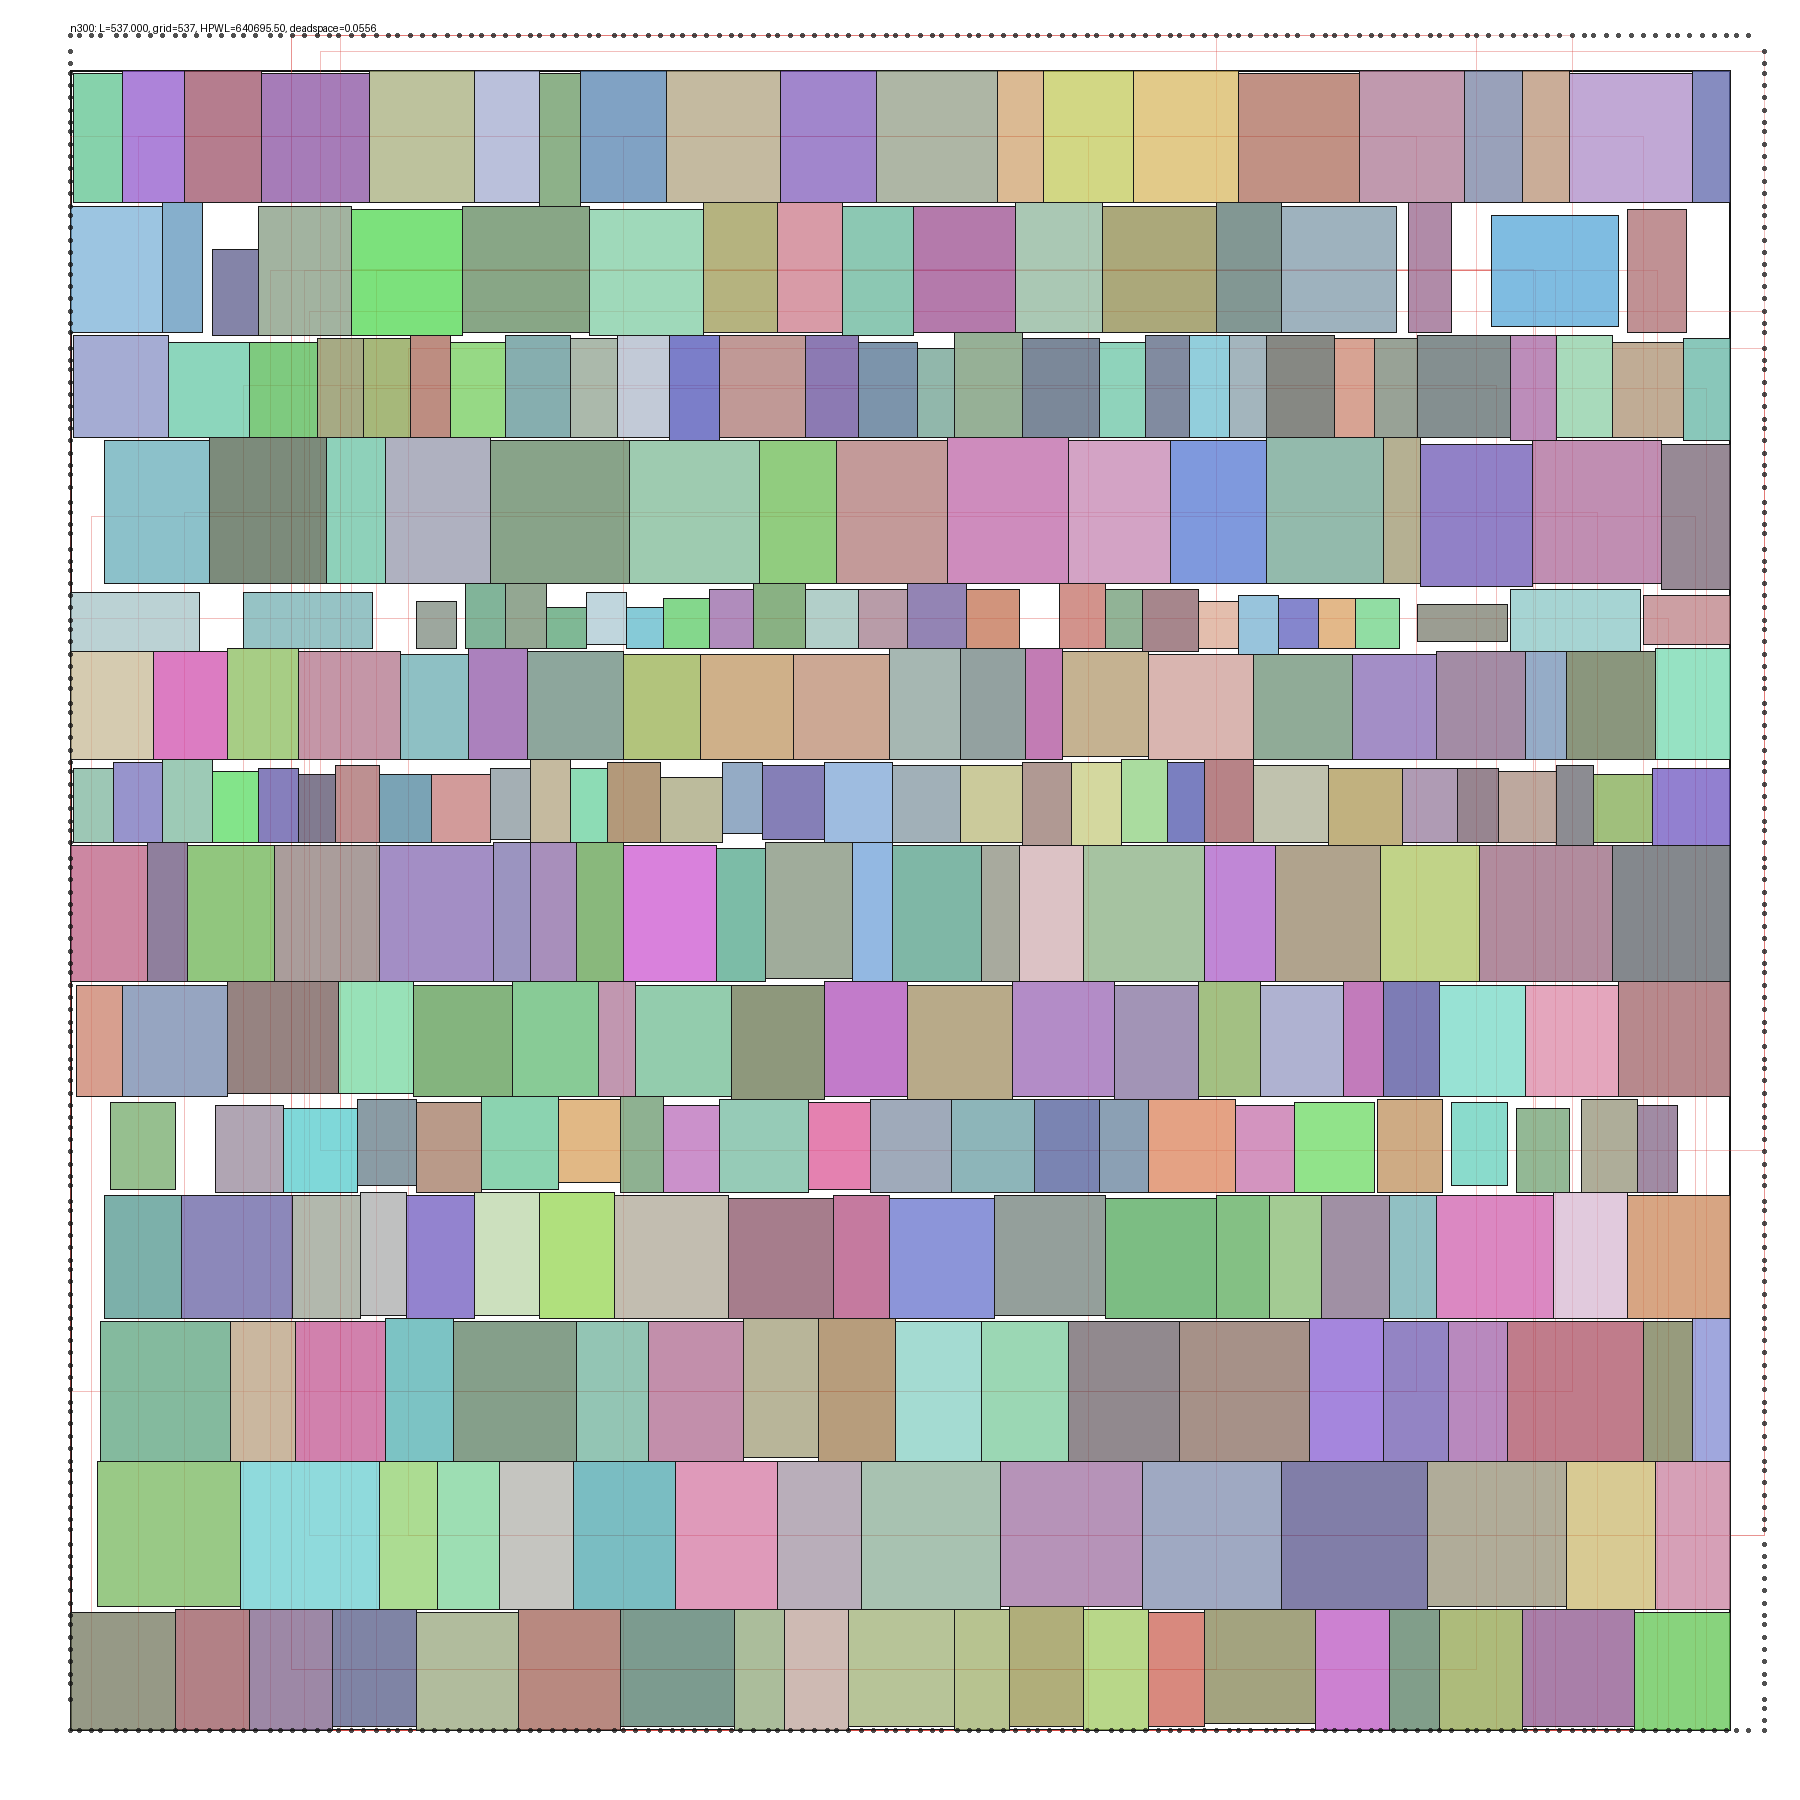
\includegraphics[width=0.76\textwidth]{../results/q3/figures/n300_q3_layout.png}
  \caption{问题三 \texttt{n300} 在边长 $537$、死区率 $5.5639\%$ 下的紧轮廓硬模块布局}
  \label{fig:q3_n300}
\end{figure}

三组布局均在压缩后的正方形内完整摆放全部硬模块。随着轮廓收紧，模块间可交换与可重插入的空间减少，布局图所呈现的高密度结构与图~\ref{fig:q3_tradeoff} 中的 HPWL 增长相互印证。

\subsection{结果检验与本问结论}

程序逐一复核模块名称完整性、轮廓边界、两两非重叠、模块总面积与 HPWL 复算一致性；三组布局均无缺失、重复、越界或重叠，且面积与线长复算结果均与表~\ref{tab:q3_main_results} 一致。完整验证计数及口径敏感性数据见附录 A.2。综上，问题三在保持布局合法的条件下，将死区率由 $15\%$ 显著压缩至 $5.5639\%$--$7.3649\%$，但相应付出了约 $7.79\%$--$14.31\%$ 的互连线长增量，清晰体现了面积利用率与互连代价之间的权衡。
